% Graphical Abstract for PatchXFormer Paper
% Compile with: pdflatex graphical_abstract.tex
\documentclass[tikz,border=10pt]{standalone}
\usepackage{tikz}
\usetikzlibrary{shapes,arrows,positioning,fit,backgrounds,shadows,decorations.pathreplacing}
\usepackage{amsmath}

\definecolor{darkblue}{RGB}{0,51,102}
\definecolor{lightblue}{RGB}{102,178,255}
\definecolor{orange}{RGB}{255,128,0}
\definecolor{green}{RGB}{34,139,34}
\definecolor{purple}{RGB}{128,0,128}
\definecolor{lightgray}{RGB}{240,240,240}

\begin{document}

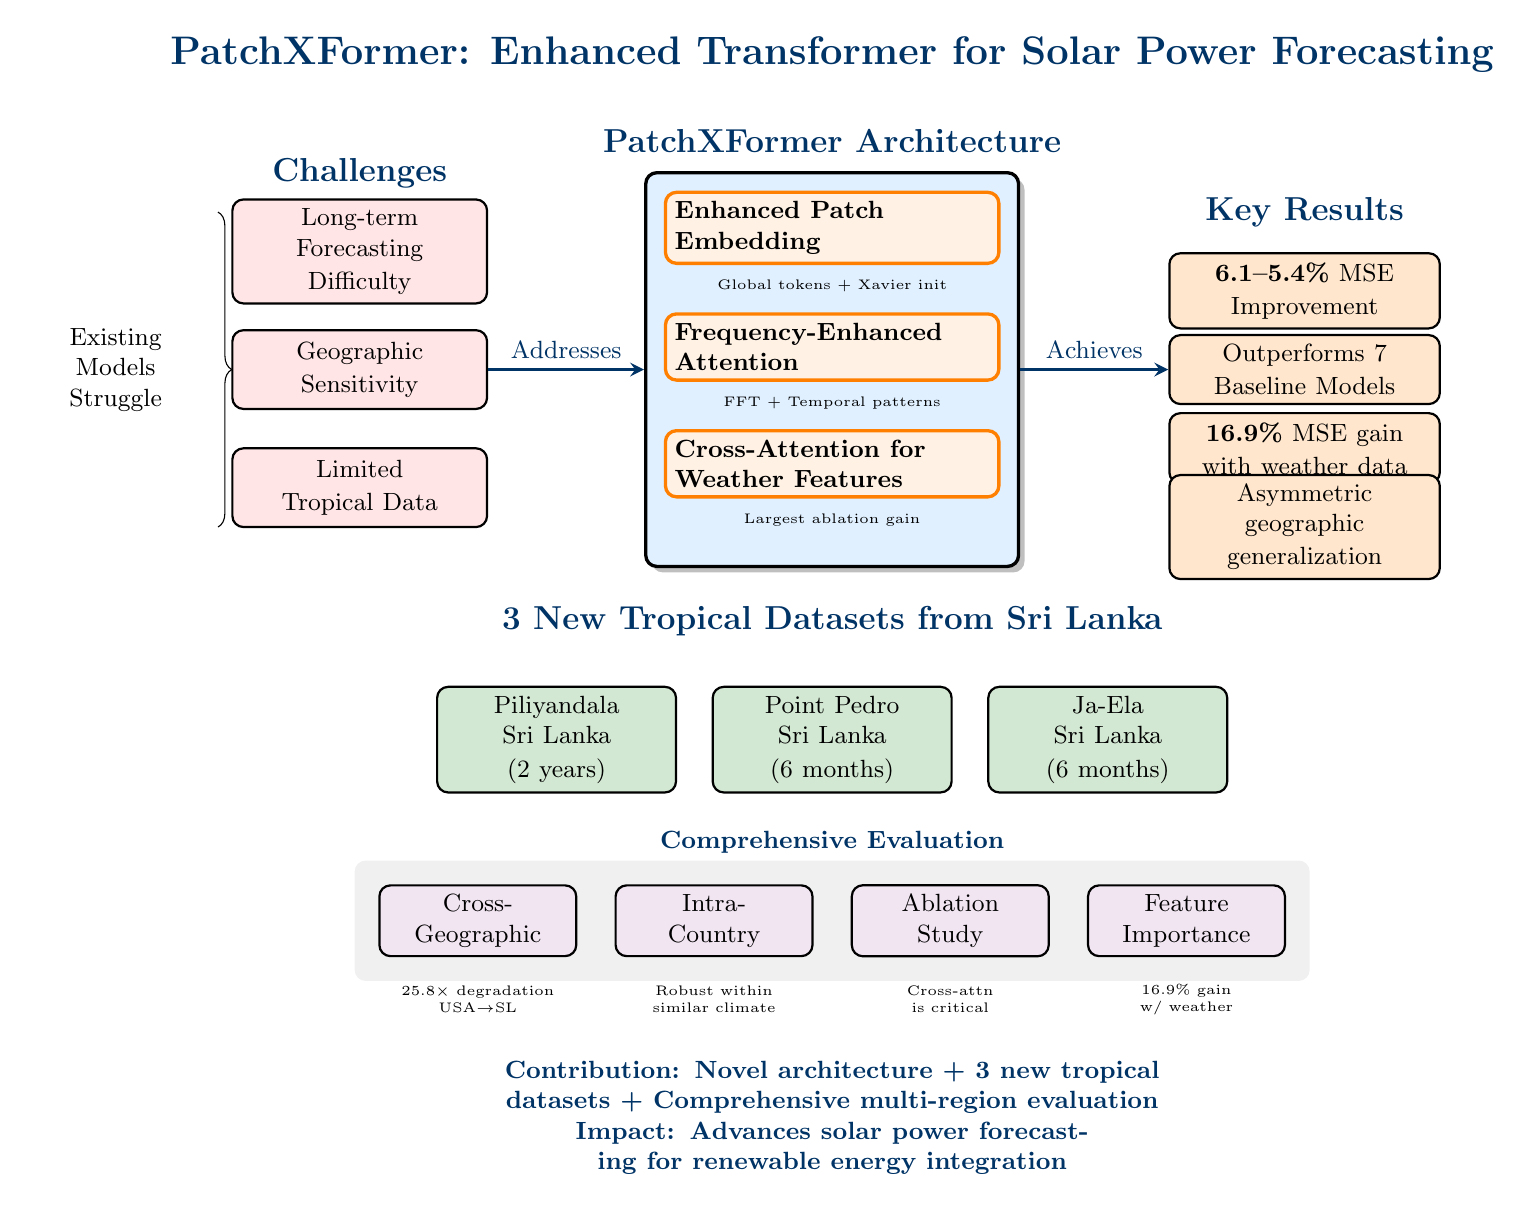
\begin{tikzpicture}[
    node distance=0.8cm,
    box/.style={rectangle, draw, thick, rounded corners, minimum width=2.5cm, minimum height=1cm, align=center, fill=white},
    bigbox/.style={rectangle, draw, very thick, rounded corners, minimum width=3.5cm, minimum height=2cm, align=center, fill=lightgray, drop shadow},
    arrow/.style={->, >=stealth, thick},
    label/.style={font=\small\bfseries},
    highlight/.style={rectangle, draw=orange, very thick, rounded corners, fill=orange!10}
]

% Title
\node[font=\Large\bfseries, darkblue] at (0,8) {PatchXFormer: Enhanced Transformer for Solar Power Forecasting};

% ------------------ Challenge Section ------------------
\begin{scope}[local bounding box=problem]
    \node[font=\large\bfseries, darkblue] at (-6,6.5) {Challenges};
    
    \node[box, fill=red!10, text width=3cm] (challenge1) at (-6,5.5) {\small Long-term\\Forecasting\\Difficulty};
    \node[box, fill=red!10, text width=3cm] (challenge2) at (-6,4) {\small Geographic\\Sensitivity};
    \node[box, fill=red!10, text width=3cm] (challenge3) at (-6,2.5) {\small Limited\\Tropical Data};
    
    \draw[decorate, decoration={brace, amplitude=5pt, mirror}] 
        (-7.8,2) -- (-7.8,6) 
        node[midway, left, xshift=-5pt, text width=2cm, align=center, font=\small] 
        {Existing\\Models\\Struggle};
\end{scope}

% ------------------ Solution Section ------------------
\node[bigbox, fill=lightblue!20, text width=4.5cm, minimum height=5cm] (mainarch) at (0,4) {};

\node[font=\large\bfseries, darkblue, fill=white] at (0,6.9) {PatchXFormer Architecture};

% Enhanced Patch Embedding
\node[highlight, text width=4cm, font=\small\bfseries] (patch) at (0,5.8) 
{Enhanced Patch\\Embedding};
\node[font=\tiny, text width=4cm, align=center, below=2pt of patch] 
{Global tokens + Xavier init};

% Frequency Attention
\node[highlight, text width=4cm, font=\small\bfseries, below=0.6cm of patch] (freq) 
{Frequency-Enhanced\\Attention};
\node[font=\tiny, text width=4cm, align=center, below=2pt of freq] 
{FFT + Temporal patterns};

% Cross Attention
\node[highlight, text width=4cm, font=\small\bfseries, below=0.6cm of freq] (cross) 
{Cross-Attention for\\Weather Features};
\node[font=\tiny, text width=4cm, align=center, below=2pt of cross] 
{Largest ablation gain};

% ------------------ Results Section ------------------
\begin{scope}[local bounding box=results]
    \node[font=\large\bfseries, darkblue] at (6,6) {Key Results};
    
    \node[box, fill=orange!20, text width=3.2cm, minimum height=0.6cm] (result1) at (6,5) {\small\textbf{6.1--5.4\%} MSE\\Improvement};
    \node[box, fill=orange!20, text width=3.2cm, minimum height=0.6cm] (result2) at (6,4) {\small Outperforms 7\\Baseline Models};
    \node[box, fill=orange!20, text width=3.2cm, minimum height=0.6cm] (result3) at (6,3) {\small \textbf{16.9\%} MSE gain\\with weather data};
    \node[box, fill=orange!20, text width=3.2cm, minimum height=0.6cm] (result4) at (6,2) {\small Asymmetric geographic\\generalization};
\end{scope}

% ------------------ Datasets Section ------------------
\begin{scope}[local bounding box=datasets]
    \node[font=\large\bfseries, darkblue] at (0,0.8) {3 New Tropical Datasets from Sri Lanka};
    
    \node[box, fill=green!20, text width=2.8cm] (sl1) at (-3.5,-0.7) {\small Piliyandala\\Sri Lanka\\(2 years)};
    \node[box, fill=green!20, text width=2.8cm] (sl2) at (0,-0.7) {\small Point Pedro\\Sri Lanka\\(6 months)};
    \node[box, fill=green!20, text width=2.8cm] (sl3) at (3.5,-0.7) {\small Ja-Ela\\Sri Lanka\\(6 months)};
\end{scope}

% ------------------ Arrows ------------------
\draw[arrow, very thick, darkblue] (challenge2) -- (mainarch.west) node[midway, above, font=\small] {Addresses};
\draw[arrow, very thick, darkblue] (mainarch.east) -- (result2.west) node[midway, above, font=\small] {Achieves};

% ------------------ Evaluation Section ------------------
\node[font=\small\bfseries, darkblue] at (0,-2.0) {Comprehensive Evaluation};

\node[box, fill=purple!10, text width=2cm, minimum height=0.6cm, font=\small] (eval1) at (-4.5,-3) {Cross-\\Geographic};
\node[box, fill=purple!10, text width=2cm, minimum height=0.6cm, font=\small] (eval2) at (-1.5,-3) {Intra-\\Country};
\node[box, fill=purple!10, text width=2cm, minimum height=0.6cm, font=\small] (eval3) at (1.5,-3) {Ablation\\Study};
\node[box, fill=purple!10, text width=2cm, minimum height=0.6cm, font=\small] (eval4) at (4.5,-3) {Feature\\Importance};

\node[font=\tiny, text width=2cm, align=center] at (-4.5,-4) {25.8$\times$ degradation\\USA$\rightarrow$SL};
\node[font=\tiny, text width=2cm, align=center] at (-1.5,-4) {Robust within\\similar climate};
\node[font=\tiny, text width=2cm, align=center] at (1.5,-4) {Cross-attn\\is critical};
\node[font=\tiny, text width=2cm, align=center] at (4.5,-4) {16.9\% gain\\w/ weather};

\begin{pgfonlayer}{background}
    \node[fit=(eval1)(eval2)(eval3)(eval4), fill=lightgray, rounded corners, inner sep=0.3cm] {};
\end{pgfonlayer}

% ------------------ Bottom Summary ------------------
\node[font=\small\bfseries, darkblue, text width=12cm, align=center] at (0,-5.5) {
    \textbf{Contribution:} Novel architecture + 3 new tropical datasets + Comprehensive multi-region evaluation\\
    \textbf{Impact:} Advances solar power forecasting for renewable energy integration
};

\end{tikzpicture}

\end{document}
